\chapter{Association schemes}\label{association}
Association schemes arise in group theory, graph theory, design theory, coding theory and more. For example, if $X$ is a finite group with conjugacy classes $\cC[g] = \{hgh^{-1}:h\in X\}$ ($g\in X$), then the conjugacy class relations $R_g = \left\{ (a,b) \mid ab^{-1} \in \cC[g]  \right\}$ yield a 
commutative association scheme on the vertex set $X$. The orbits on $X\times X$ of any 
permutation group $G$ acting generously transitively on a set $X$  give a symmetric association scheme.
Some of the most well-studied association schemes are distance-regular graphs, including Moore graphs, distance-transitive graphs, strongly regular graphs, generalized polygons, etc. One studies 
$q$-ary error-correcting codes of length  $n$ as vertex subsets of the Hamming association scheme
$H(n,q)$ \cite[Sec.~9.2]{Brouwer1989} and one studies $t$-($v,k,\lambda$) designs as vertex subsets of the 
Johnson association scheme  $J(v,k)$ \cite[Sec.~9.1]{Brouwer1989}.  For an introduction to the 
extensive literature on the subject, the reader may consult \cite{Delsarte1973,Bannai1984,Brouwer1989,Godsil1993}, 
the survey \cite{Martin2009}, or the more recent book of  Bailey \cite{Bailey2005} which focuses on 
connections to the statistical design of experiments.

Let $X$ be a finite set of vertices. A \textit{symmetric d-class association scheme} (see \cite{Brouwer1989}) on $X$ is a pair $\mathcal{L} = (X,\mathcal{R})$ where $\mathcal{R} =\left\{R_0,R_1,\dots,R_d\right\}$ is a set of $d+1$ relations on $X$ satisfying the following properties:
\begin{enumerate}[label=(\roman*)]
	\item $R_0$ is the identity relation;
	\item $\left\{R_0,R_1,\dots, R_d\right\}$ forms a partition of $X\times X$;
	\item $(x,y)\in R_i$ implies $(y,x)\in R_i$;
	\item for $0\leq i,j,k\leq d$ there exist constants $p_{i,j}^k$ such that for any $(x,y)\in R_k$, the number of vertices $z$ for which $(x,z)\in R_i$ and $(z,y)\in R_j$ is equal to $p_{i,j}^k$ independent of our original choice of $x$ and $y$.
\end{enumerate}
The constants $p_{i,j}^k$ are known as the \emph{intersection numbers} of our association scheme and we allow ourselves to suppress the comma whenever $i$ and $j$ are given by single digits, thus $p_{0,7}^6$ and $p_{07}^6$ synonymous but we will never write $p_{102}^2$, instead using $p_{10,2}^2$. Property $(iii)$ and $(iv)$ together imply that $p_{ij}^k = p_{ji}^k$ for all $i,j,k$, thus any symmetric association schemes will be \textit{commutative}. There is a broader definition for an association scheme where we replace $(iii)$ with the requirement that for every $i$, there exists some $j$ such that $R_j = R_i^T$; that is $(x,y)\in R_i$ if and only if $(y,x)\in R_j$. In this case however, we add the additional requirement $p_{ij}^k = p_{ji}^k$ so that our scheme remains commutative. Throughout this text, all association schemes will be symmetric and therefore commutative, but we will add remarks at times when the theorems may be extended to the non-symmetric case.

For each $0\leq i\leq d$ we define the (undirected) graph $\Gamma_i = \Gamma(X,R_i)$ on $X$ with $\Gamma_1,\dots,\Gamma_d$ all simple. For each $a\in X$ we define the $i^\text{th}$ \emph{neighborhood} of $a$ $R_i(a) = \left\{b\in X\vert (a,b)\in R_i\right\}$; i.e. $R_i(a)$ is the neighborhood of $a$ in the graph $\Gamma_i$. Then for any $a\in X$, the set $X$ is partitioned into the \emph{subconstituents} $R_i(a)$ for $0\leq i\leq d$. Consider the following example on $8$ vertices:
\begin{example} Consider the association scheme called the \emph{3-cube} on vertex set $X = \left\{1,\dots,8\right\}$ with relations corresponding to the graphs $\Gamma_0,\dots,\Gamma_3$ given below.
	\begin{figure}[H]\begin{center}\scalebox{.7}{$\begin{aligned}
	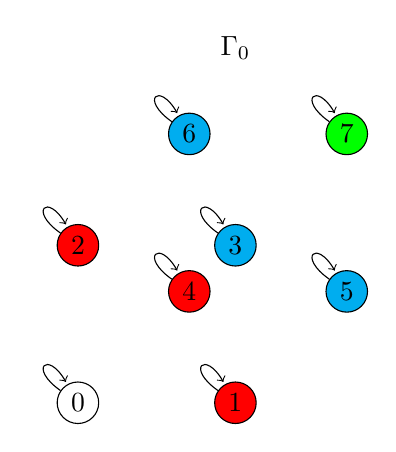
\begin{tikzpicture}[shorten >=1pt,auto,node distance=2cm,
	thin,main node/.style = {circle,draw, inner sep = 0pt, minimum size = 15pt}]
	
	\node[main node,fill=white] (1) {0};
	\node[main node,fill=red] [right of = 1](2) {1};
	\node[main node,fill=red] [above of = 1](3) {2};
	\node[main node,fill=cyan] [right of = 3](4) {3};
	\node[main node,fill=red] [above right of = 1](5) {4};
	\node[main node,fill=cyan] [right of = 5](6) {5};
	\node[main node,fill=cyan] [above of = 5] (7) {6};
	\node[main node,fill=green] [right of = 7](8) {7};
	\node at (2,4.5) (9) {$\Gamma_0$};
	
	\path (1) edge [in=120,out=145,loop] ();
	\path (2) edge [in=120,out=145,loop] ();
	\path (3) edge [in=120,out=145,loop] ();
	\path (4) edge [in=120,out=145,loop] ();
	\path (5) edge [in=120,out=145,loop] ();
	\path (6) edge [in=120,out=145,loop] ();
	\path (7) edge [in=120,out=145,loop] ();
	\path (8) edge [in=120,out=145,loop] ();
	
	\end{tikzpicture}\qquad&\qquad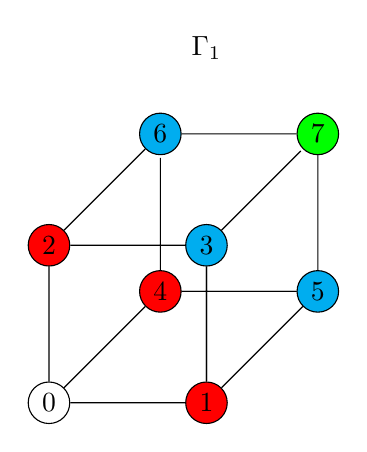
\begin{tikzpicture}[shorten >=1pt,auto,node distance=2cm,
	thin,main node/.style = {circle,draw, inner sep = 0pt, minimum size = 15pt}]
	
	\node[main node,fill=white] (1) {0};
	\node[main node,fill=red] [right of = 1](2) {1};
	\node[main node,fill=red] [above of = 1](3) {2};
	\node[main node,fill=cyan] [right of = 3](4) {3};
	\node[main node,fill=red] [above right of = 1](5) {4};
	\node[main node,fill=cyan] [right of = 5](6) {5};
	\node[main node,fill=cyan] [above of = 5] (7) {6};
	\node[main node,fill=green] [right of = 7](8) {7};
	\node at (2,4.5) (9) {$\Gamma_1$};
	
	\draw[-] (3)--(1)--(2)--(4)--(3)--(7)--(8)--(6)--(5)--(7);
	\draw[-] (1)--(5)--(6)--(2)--(4)--(8);
	\end{tikzpicture}\qquad\qquad
	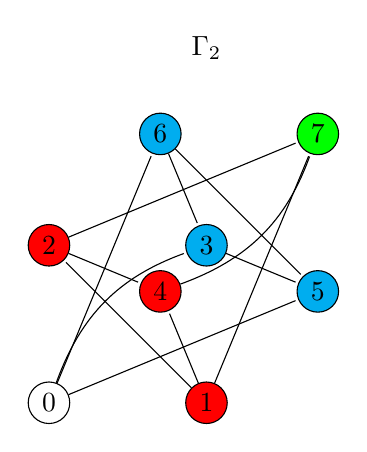
\begin{tikzpicture}[shorten >=1pt,auto,node distance=2cm,
	thin,main node/.style = {circle,draw, inner sep = 0pt, minimum size = 15pt}]
	
	\node[main node,fill=white] (1) {0};
	\node[main node,fill=red] [right of = 1](2) {1};
	\node[main node,fill=red] [above of = 1](3) {2};
	\node[main node,fill=cyan] [right of = 3](4) {3};
	\node[main node,fill=red] [above right of = 1](5) {4};
	\node[main node,fill=cyan] [right of = 5](6) {5};
	\node[main node,fill=cyan] [above of = 5] (7) {6};
	\node[main node,fill=green] [right of = 7](8) {7};
	\node at (2,4.5) (9) {$\Gamma_2$};
	
	\path[-]
	(1)edge [bend left=25] node {} (4)
	edge node {} (6)
	edge node {} (7)
	(2)edge node {} (3)
	edge node {} (5)
	edge node {} (8)
	(3)edge node {} (5)
	edge node {} (8)
	(4) edge node {} (6)
	(7) edge node {} (4)
	edge node {} (6)
	(5) edge [bend right = 25] node {} (8);
	\end{tikzpicture}\qquad&\qquad
	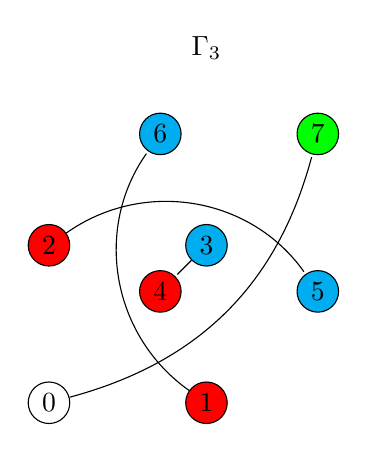
\begin{tikzpicture}[shorten >=1pt,auto,node distance=2cm,
	thin,main node/.style = {circle,draw, inner sep = 0pt, minimum size = 15pt}]
	
	\node[main node,fill=white] (1) {0};
	\node[main node,fill=red] [right of = 1](2) {1};
	\node[main node,fill=red] [above of = 1](3) {2};
	\node[main node,fill=cyan] [right of = 3](4) {3};
	\node[main node,fill=red] [above right of = 1](5) {4};
	\node[main node,fill=cyan] [right of = 5](6) {5};
	\node[main node,fill=cyan] [above of = 5] (7) {6};
	\node[main node,fill=green] [right of = 7](8) {7};
	\node at (2,4.5) (9) {$\Gamma_3$};
	
	\path[-]
	(1) edge [bend right] node {} (8)
	(2) edge [bend left=45] node {} (7)
	(3) edge [bend left=45] node {} (6)
	(4) edge node {} (5);
	\end{tikzpicture}
	\end{aligned}$}\end{center}
	\caption[Graphs of the 3-cube.]{The four graphs of the 3-cube. The four subconstituents of the vertex $0$ are colored white, red, blue, and green respectively.}\label{3cube}
	\end{figure}
	The intersection numbers of this association scheme are as follows where the $i^\text{th}$ matrix list $p^k_{ij}$ with rows indexed by $k$ and columns indexed by $j$:
	\[\left[\begin{array}{cccc}
	1&0&0&0\\
	0&1&0&0\\
	0&0&1&0\\
	0&0&0&1\\
	\end{array}\right],\left[\begin{array}{cccc}
	0&3&0&0\\
	1&0&2&0\\
	0&2&0&1\\
	0&0&3&0\\
	\end{array}\right],\left[\begin{array}{cccc}
	0&0&3&0\\
	0&2&0&1\\
	1&0&2&0\\
	0&3&0&0\\
	\end{array}\right],\left[\begin{array}{cccc}
	0&0&0&1\\
	0&0&1&0\\
	0&1&0&0\\
	1&0&0&0\\
	\end{array}\right].\]
	Since $p^k_{ij} = p^k_{ji}$ we note that many of the columns listed above are repeated, thus we may instead give a more brief list of the intersection numbers as follows:
	\[\begin{array}{c|cccc|ccc|cc|c}
	j & p^{j}_{0,0}	&p^{j}_{0,1}& p^{j}_{0,2} 	& p^{j}_{0,3}   & p^{j}_{1,1}	&p^{j}_{1,2}& p^{j}_{1,3} 	& p^{j}_{2,2} 	& p^{j}_{2,3} 	& p^{j}_{3,3}\\\hline
	0 & 1			& 0			& 0 			& 0				& 3				& 0			& 0 			& 3				& 0   			& 1\\
	1 & 0			& 1			& 0 			& 0				& 0				& 2			& 0 			& 0   			& 1   			& 0\\
	2 & 0			& 0			& 1 			& 0				& 2				& 0 		& 1				& 2 			& 0 			& 0\\
	3 & 0			& 0			& 0 			& 1				& 0 			& 3			& 0 			& 0   			& 0 			& 0\\
	\end{array}\]
	We will often find this brief description useful and will further reduce our description of the parameters in many of the examples we give where possible.
\end{example}
For any $0\leq i\leq d$ and any vertex $x\in X$,
\[p^{0}_{ii} = \left\vert\left\{y:(y,x)\in R_i\right\}\right\vert = \left\vert R_i(x)\right\vert.\]
Thus we define $k_i:=p^0_{ii}$ as the \emph{valency} of the $i^\text{th}$ relation. Many other restrictions on our intersection numbers follows immediately from our definition, for instance $p^0_{12} = 0$; we will summarize these in a latter lemma.
\section{Bose-Mesner algebra}
Often it becomes useful to order the vertices in $X$ and then represent each $R_i$ as a 01-matrix $A_i$ where the $(x,y)$ entry of $A_i$ is 1 if and only if $(x,y)\in R_i$, thus $A_i$ is the adjacency matrix of $\Gamma_i$. The defining properties of an association scheme are then encoded as:
\begin{enumerate}[label=(\roman*)]
	\item $A_0 = I$;
	\item $\sum_i A_i = J$;
	\item for all $0\leq i\leq d$, $A_i^T = A_i$;
	\item for all $0\leq i,j\leq d$, $A_iA_j = \sum p_{i,j}^k A_k$.
\end{enumerate}
The fourth condition tells us that $\BMA = \text{span}\left\{A_0,A_1,\dots A_d\right\}$ forms a matrix algebra under standard matrix multiplication. We call this algebra the \emph{Bose-Mesner algebra} and note that the remaining conditions ensure it is a $(d+1)$-dimensional algebra of symmetric matrices containing the identity. Further, as our basis matrices are 01-matrices with disjoint support, this algebra is also closed under Schur (element-wise) products. Since $p^k_{ij} = p^k_{ji}$ for all $i,j,k$, we must have $A_iA_j = A_jA_i$, that is our algebra is also commutative. Therefore we may simultaneously diagonalize the matrices $\left\{A_0,\dots,A_d\right\}$ using the maximal common orthogonal eigenspaces $V_0,\dots,V_{d'}$ with corresponding idempotents $E_0,\dots,E_{d'}$. Since, for every $i$, there exists eigenvalues $\theta_{ij}$ such that $A_i = \sum_{j=0}^{d'}\theta_{ij}E_j$ we find that $\BMA \subseteq \text{span}\left\{E_0,E_1,\dots, E_{d'}\right\}$ thus $d\leq d'$. Further since the eigenspaces $V_j$ are maximal for each $0\leq j\leq d$ and pairwise orthogonal,
\[E_j = \frac{1}{c_j}\prod_{i=0}^d\left(\prod_{\theta_{ik}\neq\theta_{ij}}\left(A_i-\theta_{ik}I\right)\right)\]
for some normalization constant $c_j$. Thus $E_j\in \BMA$ giving $\text{span}\left\{E_0,E_1,\dots, E_{d'}\right\}\subseteq\BMA$ and therefore $d=d'$. Then, for any $d$-class association scheme there is a basis of exactly $d+1$ idempotents $E_0,\dots,E_d$ which are unique up to reordering and diagonalize every matrix in $\BMA$. Since $J\in\BMA$, the rank 1 idempotent $\frac{1}{\vert X\vert}J$ must be contained within this basis; by convention we assume $E_0= \frac{1}{\vert X\vert}J$. We take a moment here to remark on the notion of duality in our matrix algebra. We have already mentioned that $\BMA$ is closed under two distinct products: standard matrix multiplication and Schur multiplication. While it is clear these are distinct products, consider an abstract vector space with basis vectors $\left\{b_i\right\}$. For any pair of vectors $v = \sum_i v_ib_i$ and $w = \sum_i w_ib_i$, we may define the \emph{product with respect to basis $\left\{b_i\right\}$} as $v\star w = \sum_i (v_iw_i)b_i$. In this light, our two distinct products become very similar; for $F,F'\in\BMA$ with $F = \sum_if_iE_i = \sum_i g_iA_i$ and $F' = \sum_if_i'E_i = \sum_i g_i'A_i$, we have
\[\begin{aligned}
FF' & =\sum_i\sum_jf_if_j'E_iE_j = \sum_i f_if_i'E_i,\\
F\circ F' &=\sum_i\sum_jg_ig_i'A_i\circ A_j= \sum_i g_ig_i'A_i.
\end{aligned}\]
Therefore our distinct products may be described as the product with respect to the basis $\left\{E_i\right\}$ (standard matrix multiplication) and the product with respect to the basis $\left\{A_i\right\}$ (elementise multiplication). Thus we consider our two products similar and will often refer to them as dual operations on our algebra. Further, we consider the basis matrices $A_0,\dots,A_d$ and $E_0,\dots,E_d$ ``dual" in a sense. Throughout this work, we will often be interested in investigating this duality and pointing out when there are differences and/or gaps in our understanding of the landscape. Our first consideration regarding these two bases for our algebra is the change of basis matrices between the two. Since both $\left\{A_0,\dots,A_d\right\}$ and $\left\{E_0,\dots,E_d\right\}$ form bases $\BMA$, there exists unique matrices $P$ and $Q$ so that
\begin{equation}
\label{PQmat}
A_i = \sum_{j} P_{ji} E_j,\qquad E_j = \frac{1}{\vert X\vert} \sum_{i} Q_{ij}A_i.
\end{equation}
We call $P$ and $Q$ the first and second eigenmatrices, noting that the eigenvalues of $A_i$ are given by column $i$ of $P$ and the ``dual eigenvalues" of $\vert X\vert E_j$, that is eigenvalues with respect to the Schur product, are given by column $j$ of $Q$. Let $\Delta_m=\text{diag}(m_0,m_1,\dots,m_d)$ and $\Delta_k=\text{diag}(k_0,k_1,\dots,k_d)$ and the following two relations hold for our eigenmatrices:
\begin{lem}[\cite{Brouwer1989}, First and second orthogonality relations] The matrices $P$ and $Q$ of an association scheme satisfy:
	\begin{equation}
	PQ = \vert X\vert I, \qquad \Delta_mP = Q^T\Delta_k
	\end{equation}
\end{lem}
A second consideration for our dual bases is that while we used the existence of structure constants $p^k_{ij}$ to show that $\BMA$ was closed under matrix multiplication, closure under Schur products came from the fact that each $A_i$ was idempotent under this product. This additional closure implies the existence of structure constants for our second basis. That is, for $0\leq i,j,k\leq d$ there exists constants $q^k_{ij}$ so that
\begin{equation}E_i\circ E_j = \frac{1}{\vert X\vert}\sum_k q_{i,j}^k E_k.\label{Emult}\end{equation}
We call these constants the \emph{Krein paramters} of the association scheme. Here we list many of the properties of both the intersection numbers and the Krein parameters, including our first and second eigenmatrices as well. See lemmas 2.1.1, 2.2.1, and 2.3.1 for proofs of the following lemma.
\begin{lem}[{\cite{Brouwer1989}}]\label{kitchensink} The parameters $p^\ell_{ij}$, $q^\ell_{ij}$, $k_i = p^0_{ii}$, $m_j = q^0_{jj}$, and the eigenmatrices $P$ and $Q$ satisfy:
	\begin{multicols}{2}
	\begin{enumerate}
		\item[(i)] $p_{0j}^\ell = \delta_{j\ell}$,
		\item[(ii)] $p^0_{ij} = \delta_{ij}k_i$,
		\item[(iii)] $p^\ell_{ij} = p^\ell_{ji}$,
		\item[(iv)] $p^\ell_{ij}k_\ell= p^j_{i\ell}k_j$,
		\item[(v)] $\sum_jp^\ell_{ij} = k_j$,
		\item[(vi)] $\sum_\ell p^\ell_{ij}p^m_{\ell h} = \sum_\ell p^m_{i\ell}p^\ell_{jh}$.
		\item[(vii)] $P_{ij}P_{ih} = \sum_\ell p^\ell_{jh}P_{i\ell}$,
		\item[(viii)] $P_{ji}Q_{hj} = \sum_\ell p_{i\ell}^hQ_{\ell j}$,
		\item[(ix)] $\sum_{j}P_{ji} = \sum_{h}p^h_{hi}$,
		\item[(x)] $P_{j0} = 1$,
		\item[(xi)] $P_{0i} = k_i$,
		\item[(xii)] $\sum_j m_jP_{ji}P_{jh} = \vert X\vert k_i\delta_{ih}$,
			
		\item[($i^\prime$)] $q^\ell_{0j} = \delta_{j\ell}$,
		\item[($ii^\prime$)] $q^0_{ij} = \delta_{ij}m_j$,
		\item[($iii^\prime$)] $q^{\ell}_{ij} = q^\ell_{ji}$,
		\item[($iv^\prime$)] $q^\ell_{ij}m_\ell = q^j_{i\ell}m_j$,
		\item[($v^\prime$)] $\sum_j q^\ell_{ij} = m_i$,
		\item[($vi^\prime$)] $\sum_\ell q^\ell_{ij}q^{m}_{\ell k} = \sum_\ell q^m_{i\ell}q^\ell_{jk}$,
		\item[($vii^\prime$)] $Q_{ij}Q_{ih} = \sum_{\ell}q^\ell_{jh}Q_{i\ell}$,
		\item[($viii^\prime$)] $P_{ij}Q_{jh} = \sum_\ell q^i_{h\ell}P_{\ell j}$,
		\item[($ix^\prime$)] $\sum_{j}Q_{ji} = \sum_{h}q^h_{hi}$,
		\item[($x^\prime$)] $Q_{i0} = 1$,
		\item[($xi^\prime$)] $Q_{0j} = m_j$,
		\item[($xii^\prime$)] $\sum_j k_iQ_{ij}Q_{ih} = \vert X\vert m_j\delta_{jh}$,
	\end{enumerate}
	\end{multicols}
\end{lem}
\section{Parameter arrays}
For a matrix $A$, we denote the entry in row $i$ and column $j$ as $\left[A\right]_{ij}$. We define the \emph{arrays of intersection numbers} $L_0,\dots,L_d$ as $(d+1)\times(d+1)$ matrices where $\left[L_i\right]_{k,j} = p^k_{ij}$. We then define the vector space $\bbL = \text{span}\left\{L_0,\dots,L_d\right\}$ and note that Lemma \ref{kitchensink} $(vi)$ gives us that
\[
\left[L_iL_j\right]_{m,k} = \sum_lp^m_{il}p^l_{jk} = \sum_{l}p^l_{ij}p^m_{lk} = \sum_l p^l_{ij}\left[L_l\right]_{m,k}
\]
for $0\leq m,k\leq d$. Therefore we find that this vector space forms a matrix algebra under matrix multiplication via
\begin{equation}\label{Lprod}
L_iL_j = \sum_l p^l_{ij}L_l.
\end{equation}
Likewise we define the \emph{arrays of Krein parameters} as $L_0^*,\dots,L_d^*$ with $\left[L_i^*\right]_{k,j} = q^k_{ij}$. This provides a dual matrix algebra $\bbL^* = \text{span}\left\{L_0^*,\dots,L_d^*\right\}$ as Lemma \ref{kitchensink} $(vi^\prime)$ gives
\begin{equation}\label{Lstarprod}
L_i^*L_j^* = \sum_{l}q^l_{ij}L_l^*.
\end{equation}
In both cases, we may define an algebra isomorphism $\phi:\BMA\rightarrow\bbL$ or $\phi^*:\BMA\rightarrow\bbL^*$ via the basis mappings
\begin{equation}
	\phi(A_i) = L_i\qquad \phi^*(E_i) = L_i^*.
\end{equation}
Note that the first isomorphism preserves standard matrix multiplication while the second preserves Schur products. We will refer to $L_1$ as the \emph{intersection matrix} and $L_1^*$ as the \emph{Krein matrix}. These these two matrices will become especially important for polynomial schemes (see Section \ref{ppoly} and \ref{qpoly}) where they are tridiagonal. We end this section by noting that the matrices given in Example \ref{3cube} were exactly the arrays of intersection numbers for that association scheme. A final note before moving on is that the parameters of an association scheme need not define the scheme uniquely. In fact, there exists non-isomorphic $2$-class association schemes with exactly the same parameters--consider the $4\times 4$ rook graph and Shrikhande graph.
\section{Example Duality}\label{dualpair}
In this section, we give an explicit example of the duality mentioned previously. Consider first the strongly regular graph given by $K_{3,3}$. This corresponding association scheme is a 2-class bipartite scheme with nontrivial relations given by adjacency in $K_{3,3}$ and non-adjacency in $K_{3,3}$ respectively. Thus the three graphs for this scheme are as follows:
	\begin{figure}[H]\begin{center}\scalebox{.7}{$\begin{aligned}
			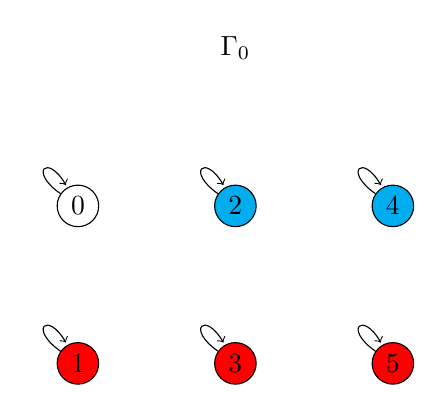
\begin{tikzpicture}[shorten >=1pt,auto,node distance=2cm,
			thin,main node/.style = {circle,draw, inner sep = 0pt, minimum size = 15pt}]
			
			\node[main node,fill=white] (1) {0};
			\node[main node,fill=cyan] [right of = 1](2) {2};
			\node[main node,fill=cyan] [right of = 2](3) {4};
			\node[main node,fill=red] [below of = 1](4) {1};
			\node[main node,fill=red] [right of = 4](5) {3};
			\node[main node,fill=red] [right of = 5](6) {5};
			\node [above of =2] (9) {$\Gamma_0$};
			
			\path (1) edge [in=120,out=145,loop] ();
			\path (2) edge [in=120,out=145,loop] ();
			\path (3) edge [in=120,out=145,loop] ();
			\path (4) edge [in=120,out=145,loop] ();
			\path (5) edge [in=120,out=145,loop] ();
			\path (6) edge [in=120,out=145,loop] ();
			
			\end{tikzpicture}\qquad&\qquad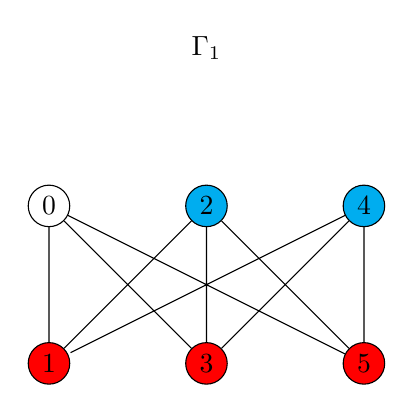
\begin{tikzpicture}[shorten >=1pt,auto,node distance=2cm,
			thin,main node/.style = {circle,draw, inner sep = 0pt, minimum size = 15pt}]
			
			\node[main node,fill=white] (1) {0};
			\node[main node,fill=cyan] [right of = 1](2) {2};
			\node[main node,fill=cyan] [right of = 2](3) {4};
			\node[main node,fill=red] [below of = 1](4) {1};
			\node[main node,fill=red] [right of = 4](5) {3};
			\node[main node,fill=red] [right of = 5](6) {5};
			\node [above of =2] {$\Gamma_1$};
			
			\draw[-] (1)--(4)--(2)--(5)--(3)--(6)--(1)--(5)--(2)--(6)--(3)--(4);
			\end{tikzpicture}\qquad\qquad
			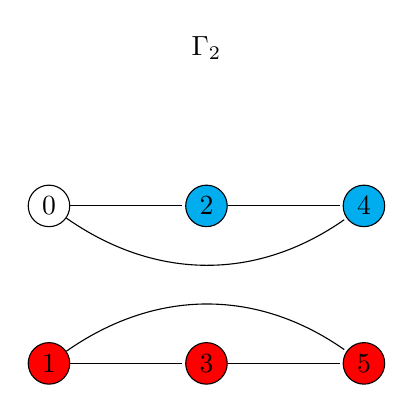
\begin{tikzpicture}[shorten >=1pt,auto,node distance=2cm,
			thin,main node/.style = {circle,draw, inner sep = 0pt, minimum size = 15pt}]	
			\node[main node,fill=white] (1) {0};
			\node[main node,fill=cyan] [right of = 1](2) {2};
			\node[main node,fill=cyan] [right of = 2](3) {4};
			\node[main node,fill=red] [below of = 1](4) {1};
			\node[main node,fill=red] [right of = 4](5) {3};
			\node[main node,fill=red] [right of = 5](6) {5};
			\node [above of =2] {$\Gamma_2$};
			
			\path[-]
			(1)edge node {} (2)
			edge [bend right=35] node {} (3)
			(2)edge node {} (3)
			(4)edge node {} (5)
			edge [bend left=35] node {} (6)
			(5) edge node {} (6);
			\end{tikzpicture}
			\end{aligned}$}\end{center}
	\caption[Graphs of $K_{3,3}$.]{The three graphs of $K_{3,3}$. The subconstituents of vertex $0$ are colored white, red,  and blue respectively.}\label{k33}
\end{figure}
The intersection numbers, Krein parameters, and eigenmatrices of this association scheme are as follows:
\[\begin{aligned}L_0 &= \left[\begin{array}{cccc}
1&0&0\\
0&1&0\\
0&0&1\\
\end{array}\right],\quad L_1 &= \left[\begin{array}{cccc}
0&3&0\\
1&0&2\\
0&3&0\\
\end{array}\right],\quad L_2 &= \left[\begin{array}{cccc}
0&0&2\\
0&2&0\\
1&0&1\\
\end{array}\right];\\
L_0^* &= \left[\begin{array}{cccc}
1&0&0\\
0&1&0\\
0&0&1\\
\end{array}\right],\quad L_1^* &= \left[\begin{array}{cccc}
0&4&0\\
1&2&1\\
0&4&0\\
\end{array}\right],\quad L_2^* &= \left[\begin{array}{cccc}
0&0&1\\
0&1&0\\
1&0&0\\
\end{array}\right];\end{aligned}\]
\[P = \left[\begin{array}{cccc}
1&3&2\\
1&0&-1\\
1&-3&2\\
\end{array}\right],\qquad Q = \left[\begin{array}{cccc}
1&4&1\\
1&0&-1\\
1&-2&1\\
\end{array}\right].\]
Now consider the second $2$-class association scheme given by the vertices of the octahedron where the two nontrivial relations are given by sharing an edge in the platonic solid and not sharing an edge respectively. The three graphs for this scheme are as follows:
\begin{figure}[H]\begin{center}\scalebox{.7}{$\begin{aligned}
			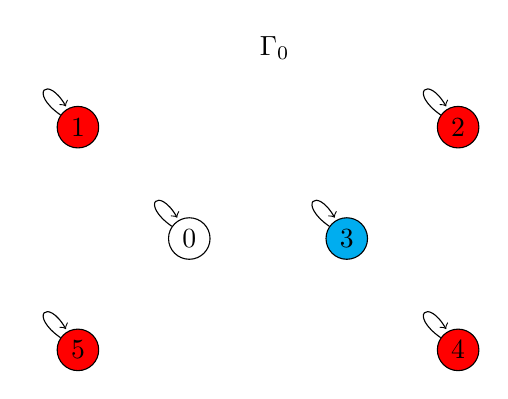
\begin{tikzpicture}[shorten >=1pt,auto,node distance=2cm,
			thin,main node/.style = {circle,draw, inner sep = 0pt, minimum size = 15pt}]
			
			\node[main node,fill=red] (2) {1};
			\node[main node,fill=white] [below right of = 2](1) {0};
			\node[main node,fill=cyan] [right of = 1](6) {3};
			\node[main node,fill=red] [above right of = 6](3) {2};
			\node[main node,fill=red] [below right of = 6](4) {4};
			\node[main node,fill=red] [below left of  = 1](5) {5};
			\node at (2.5,1) (9) {$\Gamma_0$};
			
			\path (1) edge [in=120,out=145,loop] ();
			\path (2) edge [in=120,out=145,loop] ();
			\path (3) edge [in=120,out=145,loop] ();
			\path (4) edge [in=120,out=145,loop] ();
			\path (5) edge [in=120,out=145,loop] ();
			\path (6) edge [in=120,out=145,loop] ();
			
			\end{tikzpicture}\qquad&\qquad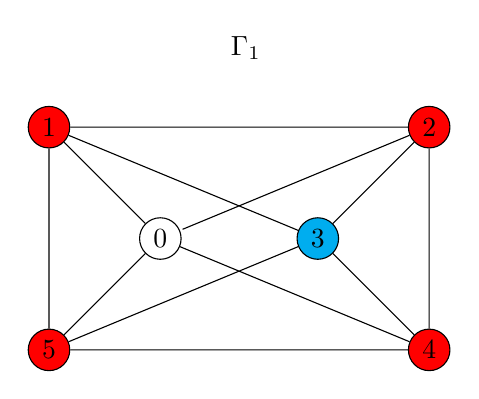
\begin{tikzpicture}[shorten >=1pt,auto,node distance=2cm,
			thin,main node/.style = {circle,draw, inner sep = 0pt, minimum size = 15pt}]
			
			\node[main node,fill=red] (2) {1};
			\node[main node,fill=white] [below right of = 2](1) {0};
			\node[main node,fill=cyan] [right of = 1](6) {3};
			\node[main node,fill=red] [above right of = 6](3) {2};
			\node[main node,fill=red] [below right of = 6](4) {4};
			\node[main node,fill=red] [below left of  = 1](5) {5};
			\node at (2.5,1) (9) {$\Gamma_1$};
			
			\draw[-] (1)--(2)--(3)--(4)--(5)--(2)--(6)--(5)--(1)--(4)--(6)--(3)--(1);
			\end{tikzpicture}\qquad\qquad
			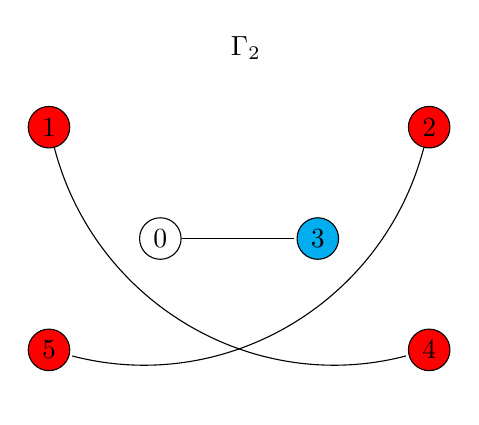
\begin{tikzpicture}[shorten >=1pt,auto,node distance=2cm,
			thin,main node/.style = {circle,draw, inner sep = 0pt, minimum size = 15pt}]	
			
			\node[main node,fill=red] (2) {1};
			\node[main node,fill=white] [below right of = 2](1) {0};
			\node[main node,fill=cyan] [right of = 1](6) {3};
			\node[main node,fill=red] [above right of = 6](3) {2};
			\node[main node,fill=red] [below right of = 6](4) {4};
			\node[main node,fill=red] [below left of  = 1](5) {5};
			\node at (2.5,1) (9) {$\Gamma_2$};
			
			\path[-]
			(1)edge node {} (6)
			(2)edge [bend right=45] node {} (4)
			(3)edge [bend left=45] node {} (5);
			\end{tikzpicture}
			\end{aligned}$}\end{center}
	\caption[Graphs of the octahedron.]{The three graphs of the octahedron. The subconstituents of vertex $0$ are colored white, red, and blue respectively.}\label{octahedron}
\end{figure}
The intersection numbers, Krein parameters, and eigenmatrices of this association scheme are as follows:
\[\begin{aligned}
L_0 &= \left[\begin{array}{cccc}
1&0&0\\
0&1&0\\
0&0&1\\
\end{array}\right],\quad L_1 &= \left[\begin{array}{cccc}
0&4&0\\
1&2&1\\
0&4&0\\
\end{array}\right],\quad L_2 &= \left[\begin{array}{cccc}
0&0&1\\
0&1&0\\
1&0&0\\
\end{array}\right];\\
L_0^* &= \left[\begin{array}{cccc}
1&0&0\\
0&1&0\\
0&0&1\\
\end{array}\right],\quad L_1^* &= \left[\begin{array}{cccc}
0&3&0\\
1&0&2\\
0&3&0\\
\end{array}\right],\quad L_2^* &= \left[\begin{array}{cccc}
0&0&2\\
0&2&0\\
1&0&1\\
\end{array}\right];
\end{aligned}\]
\[P = \left[\begin{array}{cccc}
1&4&1\\
1&0&-1\\
1&-2&1\\
\end{array}\right],\qquad Q = \left[\begin{array}{cccc}
1&3&2\\
1&0&-1\\
1&-3&2\\
\end{array}\right].\]
One may observe that the intersection numbers and the Krein parameters of the two schemes are interchanged as well as the first and second eigenmatrices. This is, in part, due to a duality arising from the context of translation schemes: schemes for which there exists an abelian group $G$ acting transitively on the vertices with $(g(x),g(y))\in R_i$ if and only if $(x,y)\in R_i$ for every $x,y\in X$ and $g\in G$. When this occurs we may define a dual association scheme (which is also a translation scheme) $(\hat{X},\hat{\mathcal{R}})$ where $\hat{X} = \left\{\chi:\chi\in G^*\right\}$ and $(\chi,\chi')\in \hat{R}_i$ if and only if $E_i (\chi-\chi') = (\chi-\chi')$. In the case of the two association schemes given above, $G\simeq Z_6$ and building the dual scheme of one will result in the other.

In general we often find the automorphism group of an association scheme to be trivial, and thus certainly do not expect to find a transitive action on the vertices. However the duality still persists at times in the formal sense. Therefore we say two association schemes are \emph{formally dual} if swaping the eigenmatrices of one gives the eigenmatrices of the other (equivalently swapping the intersection numbers and Krein parameters of one gives the parameters of the other). We often find that no dual scheme may exist (consider any association scheme for which the Krein parameters are not integral), however this notion of formal duality still plays a major role in our understanding of the field of association schemes as a whole. It will motivative many of the questions which we will focus on in this thesis. We finish this example with one final note: any parameter level definition will often bring rise to similar definitions for the dual. For instance we find that $K_{3,3}$ is bipartite because $p^k_{ij}= 0$ whenever $i+j+k\notin2\bbZ$. Then the dual graph, the octahedron, follows $q^k_{ij}=0$ whenever $i+j+k\notin2\bbZ$ and we will call this ``dual-bipartite" or $Q$-bipartite (see \ref{qbip}). Similarly we find that both $K_{3,3}$ and the octahedron are ``antipodal graphs": $p^d_{di} = 0$ whenever $i\notin\left\{0,d\right\}$. Thus both graphs are also what we call ``dual-antipodal" or $Q$-antipodal (see \ref{qant}): $q^d_{di}=0$ whenever $i\notin\left\{0,d\right\}$. While there has been much research into bipartite and antipodal graphs, in this body of work we are interested in the implications of these dual properties, seeking when such objects can exist and what structure they bring.
\section{Feasibility and Realizability}
We are often interested in whether or not an association scheme exists given a (possibly partial) parameter set. While existence often cannot be proven at the level of parameters, there are many times where we may rule out the existence of a scheme due to the values its intersection numbers or Krein parameters must take. In this section we examine three main conditions which we will use throughout this text in addition to what we already stated in Lemma \ref{kitchensink}. We begin with an immediate restriction on the intersection numbers:
\begin{lem}[\cite{Brouwer1989}]\label{intfeas}
	The intersection numbers of an association scheme must be non-negative integers.\qed
\end{lem}
This condition is easy to verify since, by definition, each $p^k_{ij}$ is the cardinality of a set. While this property is immediate, it can be a powerful tool to eliminate examples with very little information about the association scheme. Next consider the Krein parameters of our association scheme.
\begin{lem}[\cite{Scott1973},Krein conditions]\label{kreinfeas}
	The Krein parameters of an association scheme must be non-negative real numbers.
\end{lem}
\begin{proof}
	From equation \eqref{Emult}, we find that $\nicefrac{q_{ij}^0}{\vert X\vert},\dots,\nicefrac{q_{ij}^d}{\vert X\vert}$ are the eigenvalues of $E_i\circ E_j$. However $E_i\circ E_j\in \BMA$ and thus it must be symmetric and therefore all eigenvalues are real. Further, $E_i\circ E_j$ is a principle submatrix of $E_i\otimes E_j$, which has two distinct eigenvalues: $1$ and $0$. Therefore $E_i\otimes E_j$ is positive semi-definite and any principle submatrix must share the same property, forcing the eigenvalues of $E_i\circ E_j$ to be non-negative.
\end{proof}
The final feasibility condition we will list here is known as the \emph{absolute bound}.
\begin{lem}[\cite{Neumaier1981},Absolute bound]\label{absolute}
	The multiplicities $m_i$ ($0\leq i\leq d$) of a $d$-class association scheme satisfy:
	\[\sum_{q_{ij}^k\neq 0} m_k\leq\begin{cases}
	m_im_j & \text{ if }i\neq j\\
	\binom{m_i+1}{2} & \text{ if }i= j.
	\end{cases}\]
\end{lem}
\begin{proof}
	The sum on the left is the rank of $E_i\circ E_j$, a principle submatrix of $E_i\otimes E_j$ which has rank $m_im_j$. If $i=j$, $E_i\circ E_j$ is the entrywise square of $E_i$. Assume $\text{col}(E_i) = \text{span}(v_1,\dots,v_{m_i})$, then the columns of $E_i\circ E_i$ must be linear combinations of the vectors $v_j\circ v_k$ for $1\leq j\leq k\leq d$, a total of $\binom{m_i+1}{2}$ vectors.
\end{proof}
\begin{definition}
	A \emph{feasible parameter set} is a set of Krein parameters and intersection numbers such that:
	\begin{itemize}
		\item[FC1:] The Krein parameters satisfy Lemmas \ref{kreinfeas} and \ref{kitchensink},
		\item[FC2:] The intersection numbers satisfy Lemmas \ref{intfeas} and \ref{kitchensink},
		\item[FC3:] The integers $m_j = q^0_{jj}$ must satisfy Lemma \ref{absolute}.
	\end{itemize}
\end{definition}
\begin{definition}
	A feasible parameter set is \emph{realizable} if there exists an association scheme $(X,\cR)$ with the given parameter set.
\end{definition}
\begin{remark}The distinction made here is to emphasize that we are restricting the definition of ``feasible" to fulfilling only a few requirements, however there are many more restrictions which must be fulfilled in any given case. For instance another immediate restriction is that $p^i_{ii}k_i$ must be even for $0\leq i\leq d$, else the graphs violate the handshaking lemma. Thus we are not making claims as to which restrictions are fundamental and merely defining a baseline of requirements which we will refer to many times in this body of work.
\end{remark}
\section{Imprimitivity}
An association scheme $(X,\cR)$ is called \emph{imprimitive} if there exists a non-trivial union of relations which results in an equivalence relation. For instance, consider the association scheme $K_{3,3}$ depicted in Figure \ref{k33} and note that the relations $R_0$ and $R_2$ together create an equivalence relation with two equivalence classes. When this occurs we call the set of relations which form the equivalence relation a \emph{system of imprimitivity} and denote the set of corresponding indices by $\cI$. In some cases, we may have multiple systems of imprimitivity in our association scheme. For instance consider Example \ref{3cube} and note that $\cI_1 = \left\{0, 2\right\}$ and $\cI_2 = \left\{0, 3\right\}$ are both systems of imprimitivity yet $\cI_1$ admits two equivalence classes while $\cI_2$ admits four. Thus we must be careful to distinguish between distinct systems of imprimitivity for any given association scheme. In each case however, we find that the size of any equivalence class is equal to the sum of the valencies corresponding to the indices in $\cI$. Thus in the example given above, the size of each equivalence class for $\cI_1$ is $v_0+v_2 = 4$, likewise the size of each equivalence class for $\cI_2$ is $v_0+v_3 = 2$. For all that follows we denote the size of any given equivalence class by $r$ and then we denote the number of equivalence classes by $w$. For each system of imprimitivity, we define two types of related association schemes: a subscheme and a quotient scheme, however we first examine the situation in general. Suppose $(X,\cR)$ is given with the system of imprimitivity $\cI = \left\{0,i_1,\dots,i_s\right\}$ and equivalence classes $X_0,X_1,\dots,X_w$. Then $\left\{A_i\right\}_{i\in\cI}$ forms a basis for a second matrix algebra $\BMA^\prime\subset\BMA$ which is also closed under both products. We may order the vertices by equivalence classes so that every matrix in $\BMA^\prime$ is block diagonal with $w$ blocks of size $r\times r$. Further, \[\left[\sum_{i\in\cI}A_i\right]_{x,y} = \begin{cases}
1 \text{ if there exists a }0\leq k\leq w\text{ with }x,y\in X_k,\\
0 \text{ otherwise.}
\end{cases}\]
Thus $\sum_{i\in\cI}A_i = I_w\otimes J_r$ under this vertex ordering. Now we may do much of the same analysis as we did with our original algebra to find a basis of idempotents $\left\{E^\prime_i\right\}_{i\in\cI}$ for $\BMA^\prime$, however each of these must be block diagonal as well with blocks of size $r\times r$. Since we have shown $I_w\otimes J_r$ is in $\BMA^\prime$, we know that $\frac{1}{r}I_w\otimes J_r$ must be one of these matrices, call it $E^\prime_0$. However since these idempotents correspond to the maximal common eigenspaces of $A_0,\dots,A_{i_s}$, every eigenspace of the original Bose-Mesner algebra must be contained within exactly one of these eigenspaces. Then for $j\in\cI$ define $\hat{j} = \left\{i:E^\prime_j E_i = E_i\right\}$. Then there exists an index set $\cJ = \hat{0}$ such that $\sum_{j\in\cJ}E_j = \frac{1}{r}I_w\otimes J_r$. The existence of such index sets $\cI$ and $\cJ$ are often used to describe the system of imprimitivity in question and both will become useful when describing the subscheme and quotient scheme. We now move to a description of these sub-objects.

\subsection*{Subscheme}
Suppose $(X,\cR)$ is given with the system of imprimitivity $\cI = \left\{0,i_1,\dots,i_s\right\}$ and equivalence classes $X_0,X_1,\dots,X_w$. Since $\cup_{i\in\cI}R_i$ is an equivalence relation, we find that for any choice of $0\leq j\leq w$ and $i\in\cI$,  $x\in X_j$ and $(x,y)\in R_i$ imply $y\in X_j$. Then for each $X_j$, we define the \emph{subscheme} of $(X,\mathcal{R})$ with respect to $\cI$ on $X_j$ as the $s$-class association scheme $\left(X_j,\left\{R_i^\prime\right\}_{i\in\cI}\right)$ on $r$ vertices where $R_i^\prime = R_i\cap\left(X_j\times X_j\right) = \left. R_i\right\vert_{X_j}$. Without loss of generality, let us consider the subscheme $\left(X_0,\left\{R_i^\prime\right\}_{i\in\cI}\right)$ with intersection numbers $\left\{p^{\prime k}_{ij}\right\}$ and Krein parameters $\left\{q^{\prime k}_{ij}\right\}$ and, following the vertex ordering from before, define $\psi:\mathbb{R}^{\vert X\vert\times \vert X\vert}\rightarrow \mathbb{R}^{r\times r}$ via $\psi(M)$ equals the top left $r\times r$ block of $M$. Then for $i\in\cI$, $A_i^\prime = \psi(A_i)$ and all remaining entries in the first $r$ rows of $A_i$ are all 0. Then $\psi(A_iA_j) = \psi(A_i)\psi(A_j)$ and we must have $p^{\prime k}_{ij} = p^k_{ij}$ for each $i,j,k\in \cI$. Further, using $\hat{j}$ defined before for $j\in\cI$, we know $E_j^\prime = \psi\left(\sum_{i\in \hat{j}}E_i\right)$ and thus
\[E_i^\prime\circ E_j^\prime = \psi\left(\sum_{\ell\in\hat{i},r\in\hat{j}}E_\ell\circ E_r\right) = \frac{1}{\vert X\vert}\psi\left(\sum_{\ell\in\hat{i},r\in\hat{j}}\sum_{k=0}^dq^k_{\ell r}E_k\right) = \frac{1}{\vert X\vert}\sum_{\hat{k}}\left(\sum_{\ell\in\hat{i},r\in\hat{j}}q^k_{\ell r}\right)\psi\left(\sum_{k\in\hat{k}}E_k\right)\]


 for $0\leq j\leq d$, $\psi(A_i)\psi(E_j) = \psi(A_i E_j) = P_{ij}\psi(E_j)$, thus each $\psi(E_j)$ is an idempotent matrix for the subscheme. Since the new Bose-Mesner algebra only has dimension $s+1$, we must have $\psi(E_j) = \psi(E_{j^\prime})$ for some $0\leq j,j^\prime\leq d$. Then, define an equivalence relation on the indices so that $i\sim j$ if and only if $\psi(E_j) = \psi(E_i)$ and define $\tilde{i} = \left\{j:j\sim i\right\}$. Then we must have $\left\vert\left\{\tilde{i}, 0\leq i\leq d\right\}\right\vert = s+1$ and for $0\leq i,j,k\leq d$ we find that
 
 
 
\[q^{\prime\tilde{k}}_{\tilde{i}\tilde{j}} = \frac{1}{\vert \tilde{k}\vert}\sum_{i\in \tilde{i},j\in\tilde{j}}q_{ij}^k.\]
For convenience, we will typically relabel the $s+1$ indices $\tilde{i}$ to $0,1,\dots,s$ when preserving the original indices is not helpful. We now consider the dual object known as the quotient scheme.
\subsection*{Quotient scheme}
Instead of defining a smaller association scheme on each of the equivalence classes, here we will define an association scheme on the equivalence classes themselves. As before suppose $(X,\cR)$ is given with the system of imprimitivity $\cI = \left\{0,i_1,\dots,i_s\right\}$ and equivalence classes $X_0,X_1,\dots,X_w$. Now, build an equivalence relation on the indices $0\leq i,j\leq d$ so that $i\sim j$ if $p^k_{ij}>0$ for some $k\in \cI$ and denote by $\tilde{i}$ the equivalence class of $i$. Note that by our definition of $\cI$, we have that $\tilde{0} = \cI$. Then we define the \emph{quotient scheme} of $(X,\mathcal{R})$ with respect to $\cI$ as $\left(\tilde{X},\tilde{\mathcal{R}}\right)$ where $\tilde{X}$ is the set of $w$ equivalence classes and $(X_i,X_j)\in \tilde{R}_{\tilde{i}}$ if there exists $x\in X_i$, $y\in X_j$, and $k\in \tilde{i}$ such that $(x,y)\in R_k$. It is less immediately clear that this fulfills our requirements for an association scheme so we verify that here. First note $(X_i,X_j)\in \tilde{R}_{\tilde{0}}$ if and only if $i=j$ since $\tilde{0} = \cI$ was an equivalence relation on the sets $X_0,\dots,X_d$, thus $\tilde{R}_{\tilde{0}}$ is the identity relation. Next for any $0\leq i,j\leq w$, $(X_i,X_j)\in \tilde{R}_{\tilde{k}}$ for some $\tilde{k}$ since both $X_i$ and $X_j$ are non-empty and $\mathcal{R}$ partitions $X\times X$. Now assume $(X_i,X_j)\in \tilde{R}_{\tilde{k}}\cap\tilde{R}_{\tilde{k'}}$. Then there exists points $x_1,x_2\in X_i$, $y_1,y_2\in X_j$ with the following relations
\[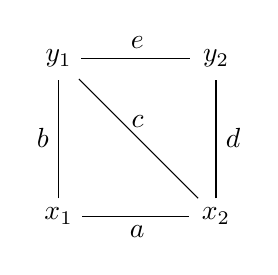
\begin{tikzpicture}[shorten >=1pt,auto,node distance=2cm,
thin,main node/.style = {circle,draw, inner sep = 0pt, minimum size = 15pt}]

\node (1) {$x_1$};
\node [right of = 1](2) {$x_2$};
\node [above of = 1](3) {$y_1$};
\node [right of = 3](4) {$y_2$};

\path[-]
(1)edge node[below] {$a$} (2)
edge node {$b$} (3)
(2)edge node[above] {$c$} (3)
edge node[right] {$d$} (4)
(3)edge node {$e$} (4);\end{tikzpicture}\]
with $a,e\in \tilde{0}$, $b\in\tilde{k}$, and $d\in\tilde{k'}$. But then $p^{a}_{bc}\geq 1$ and $p^e_{cd}\geq 1$, thus $\tilde{k} = \tilde{c} = \tilde{k'}$ and our relations must partition $\tilde{X}\times\tilde{X}$. Further, each relation $\tilde{R}_{\tilde{k}}$ is symmetric since our original relations were symmetric. Then all that is left to show is the existence of intersection numbers. One may verify that for $0\leq i,j,k\leq d$ we have
\[\tilde{p}^{\tilde{k}}_{\tilde{i}\tilde{j}} = \frac{1}{r}\sum_{i\in\tilde{i},j\in\tilde{j}} p^k_{ij}.\]


To illustrate these objects, consider the $3$-cube from before and recall there were two systems of imprimitivity: $\cI_1 = \left\{0, 2\right\}$ and $\cI_2 = \left\{0, 3\right\}$.

We begin with $\cI_1 = \left\{0,2\right\}$ and display the components of $\Gamma_2$ below.
	\begin{center}\scalebox{.7}{$\begin{aligned}
			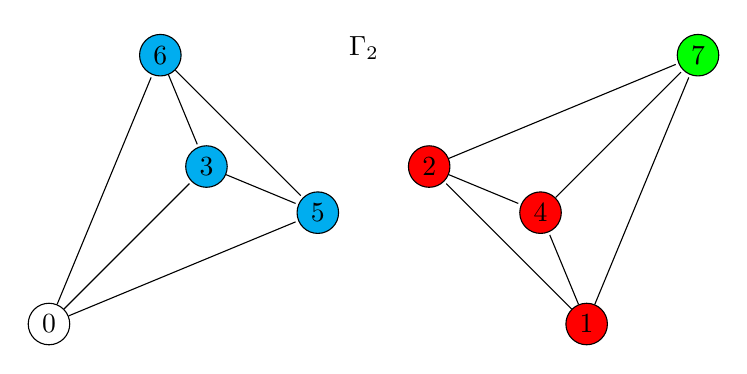
\begin{tikzpicture}[shorten >=1pt,auto,node distance=2cm,
			thin,main node/.style = {circle,draw, inner sep = 0pt, minimum size = 15pt}]
			
			\node[main node,fill=white] (1) {0};
			\node [right of = 1](2) {};
			\node [above of = 1](3) {};
			\node[main node,fill=cyan] [right of = 3](4) {3};
			\node [above right of = 1](5) {};
			\node[main node,fill=cyan] [right of = 5](6) {5};
			\node[main node,fill=cyan] [above of = 5] (7) {6};
			\node [right of = 7](8) {};
			
			\node [below right of =6] (11) {};
			\node[main node,fill=red] [right of = 11](12) {1};
			\node[main node,fill=red] [above of = 11](13) {2};
			\node [right of = 13](14) {};
			\node[main node,fill=red] [above right of = 11](15) {4};
			\node [right of = 15](16) {};
			\node [above of = 15] (17) {};
			\node[main node,fill=green] [right of = 17](18) {7};
			\node at (4,3.5) (9) {$\Gamma_2$};
			
			\path[-]
			(1)edge node {} (4)
			edge node {} (6)
			edge node {} (7)
			(12)edge node {} (13)
			edge node {} (15)
			edge node {} (18)
			(13)edge node {} (15)
			edge node {} (18)
			(4) edge node {} (6)
			(7) edge node {} (4)
			edge node {} (6)
			(15) edge node {} (18);
			\end{tikzpicture}
			\end{aligned}$}\end{center}
		Since there are two distinct components, we find two subschemes. In this case they are both isomorphic to $K_4$:	
	\begin{center}\scalebox{.7}{$\begin{aligned}
			\begin{tikzpicture}[shorten >=1pt,auto,node distance=2cm,
			thin,main node/.style = {circle,draw, inner sep = 0pt, minimum size = 15pt}]
			
			\node[main node,fill=white] (1) {0};
			\node[main node,fill=cyan] [right of = 3](4) {1};
			\node[main node,fill=cyan] [right of = 5](6) {2};
			\node[main node,fill=cyan] [above of = 5] (7) {3};
			\node at (2,4.5) (9) {$\Gamma_0^\prime$};
			
			\path (1) edge [in=120,out=145,loop] ();
			\path (4) edge [in=120,out=145,loop] ();
			\path (6) edge [in=120,out=145,loop] ();
			\path (7) edge [in=120,out=145,loop] ();
			
			\end{tikzpicture}\qquad\qquad
			\begin{tikzpicture}[shorten >=1pt,auto,node distance=2cm,
			thin,main node/.style = {circle,draw, inner sep = 0pt, minimum size = 15pt}]
			
			\node[main node,fill=white] (1) {0};
			\node[main node,fill=cyan] [right of = 3](4) {1};
			\node[main node,fill=cyan] [right of = 5](6) {2};
			\node[main node,fill=cyan] [above of = 5] (7) {3};
			\node at (2,4.5) (9) {$\Gamma_1^\prime$};
			
			\path[-]
			(1)edge node {} (4)
			edge node {} (6)
			edge node {} (7)
			(4) edge node {} (6)
			(7) edge node {} (4)
			edge node {} (6);
			\end{tikzpicture}
			\end{aligned}$}\end{center}
		Finally the quotient scheme is found by collapsing each component to a single point, giving the association scheme isomorphic to $K_2$
		\begin{center}\scalebox{.7}{$\begin{aligned}
		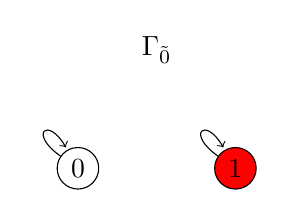
\begin{tikzpicture}[shorten >=1pt,auto,node distance=2cm,
		thin,main node/.style = {circle,draw, inner sep = 0pt, minimum size = 15pt}]
		
		\node[main node,fill=white] (1) {0};
		\node[main node,fill=red] [right of = 1](2) {1};
		\node at (1,1.5) (9) {$\Gamma_{\tilde{0}}$};
		
		\path (1) edge [in=120,out=145,loop] ();
		\path (2) edge [in=120,out=145,loop] ();
		
		\end{tikzpicture}\qquad\qquad
		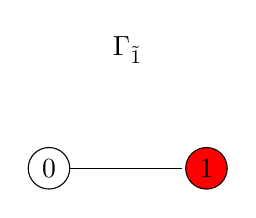
\begin{tikzpicture}[shorten >=1pt,auto,node distance=2cm,
		thin,main node/.style = {circle,draw, inner sep = 0pt, minimum size = 15pt}]
		
		\node[main node,fill=white] (1) {0};
		\node[main node,fill=red] [right of = 1](2) {1};
		\node at (1,1.5) (9) {$\Gamma_{\tilde{1}}$};
		
		\path[-]
		(1)edge node {} (2);
		\end{tikzpicture}
	\end{aligned}$}\end{center}
Similarly, if we consider the system of imprimitivity given by $\cI_2 = \left\{0,3\right\}$ then we find the components of $\Gamma_3$:
\begin{center}\scalebox{.7}{$\begin{aligned}
		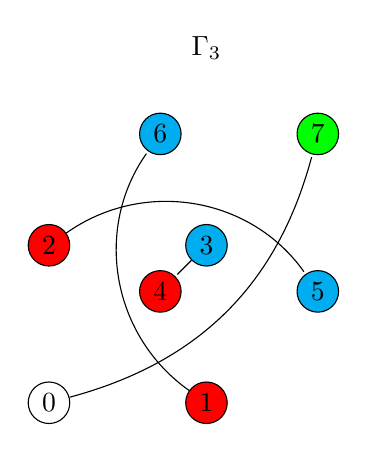
\begin{tikzpicture}[shorten >=1pt,auto,node distance=2cm,
		thin,main node/.style = {circle,draw, inner sep = 0pt, minimum size = 15pt}]
		
		\node[main node,fill=white] (1) {0};
		\node[main node,fill=red] [right of = 1](2) {1};
		\node[main node,fill=red] [above of = 1](3) {2};
		\node[main node,fill=cyan] [right of = 3](4) {3};
		\node[main node,fill=red] [above right of = 1](5) {4};
		\node[main node,fill=cyan] [right of = 5](6) {5};
		\node[main node,fill=cyan] [above of = 5] (7) {6};
		\node[main node,fill=green] [right of = 7](8) {7};
		\node at (2,4.5) (9) {$\Gamma_3$};
		
		\path[-]
		(1) edge [bend right] node {} (8)
		(2) edge [bend left=45] node {} (7)
		(3) edge [bend left=45] node {} (6)
		(4) edge node {} (5);
		\end{tikzpicture}
		\end{aligned}$}\end{center}
	These components give rise to four subschemes, each isomorphic to $K_2$:
	\begin{center}\scalebox{.7}{$\begin{aligned}
			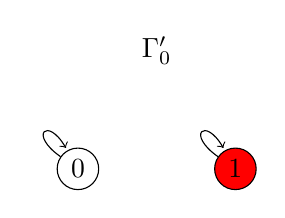
\begin{tikzpicture}[shorten >=1pt,auto,node distance=2cm,
			thin,main node/.style = {circle,draw, inner sep = 0pt, minimum size = 15pt}]
			
			\node[main node,fill=white] (1) {0};
			\node[main node,fill=red] [right of = 1](2) {1};
			\node at (1,1.5) (9) {$\Gamma_0^\prime$};
			
			\path (1) edge [in=120,out=145,loop] ();
			\path (2) edge [in=120,out=145,loop] ();
			
			\end{tikzpicture}\qquad\qquad
			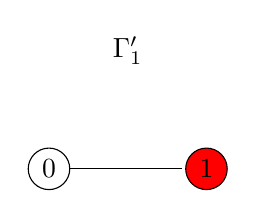
\begin{tikzpicture}[shorten >=1pt,auto,node distance=2cm,
			thin,main node/.style = {circle,draw, inner sep = 0pt, minimum size = 15pt}]
			
			\node[main node,fill=white] (1) {0};
			\node[main node,fill=red] [right of = 1](2) {1};
			\node at (1,1.5) (9) {$\Gamma_1^\prime$};
			
			\path[-]
			(1)edge node {} (2);
			\end{tikzpicture}
			\end{aligned}$}\end{center}
		Further, the quotient scheme is isomorphic to $K_4$:
		
		\begin{center}\scalebox{.7}{$\begin{aligned}
				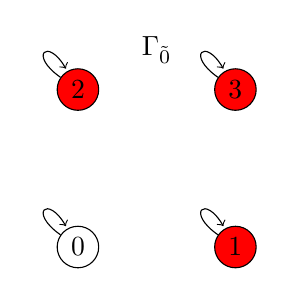
\begin{tikzpicture}[shorten >=1pt,auto,node distance=2cm,
				thin,main node/.style = {circle,draw, inner sep = 0pt, minimum size = 15pt}]
				
				\node[main node,fill=white] (1) {0};
				\node[main node,fill=red] [right of = 1](2) {1};
				\node[main node,fill=red] [above of = 1](3) {2};
				\node[main node,fill=red] [above of =2](4) {3};
				\node at (1,2.5) (9) {$\Gamma_{\tilde{0}}$};
				
				\path (1) edge [in=120,out=145,loop] ();
				\path (2) edge [in=120,out=145,loop] ();
				\path (3) edge [in=120,out=145,loop] ();
				\path (4) edge [in=120,out=145,loop] ();
				
				\end{tikzpicture}\qquad&\qquad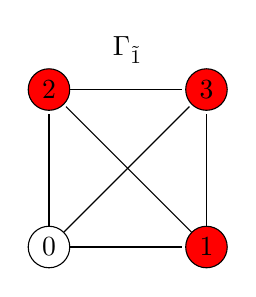
\begin{tikzpicture}[shorten >=1pt,auto,node distance=2cm,
				thin,main node/.style = {circle,draw, inner sep = 0pt, minimum size = 15pt}]
				
				\node[main node,fill=white] (1) {0};
				\node[main node,fill=red] [right of = 1](2) {1};
				\node[main node,fill=red] [above of = 1](3) {2};
				\node[main node,fill=red] [above of =2](4) {3};
				\node at (1,2.5) (9) {$\Gamma_{\tilde{1}}$};
				
				\path[-]
				(1) edge node {} (2)
				edge node {} (3)
				edge node {} (4)
				(2) edge node {} (3)
				edge node {} (4)
				(3) edge node {} (4);
				\end{tikzpicture}
				\end{aligned}$}\end{center}
We close this section by noting that the various subschemes generated by a single system of imprimitivity need not be isomorphic, despite the fact that they were for the scheme above. This is simply due to the fact that the subschemes in each case were 1-class association schemes. Instead we find that the only requirement is that the parameters of each subscheme are the same, which we have already noted does not imply the schemes are isomorphic as long as $d\geq 2$.
\section{Metric schemes}\label{ppoly}
\section{Cometric schemes}\label{qpoly}
A \textit{$Q$-polynomial} (\textit{cometric}) association scheme is one in which the set $\left\{E_0,E_1,\dots,E_d\right\}$ may be ordered so that $q^{k}_{i,j} = 0$ whenever $k>i+j$ or $k<\vert i- j\vert$ and $q^{k}_{i,j}>0$ whenever $k = i+j$. Finally, we say an association scheme with $Q$-polynomial ordering $E_0,\dots,E_d$ is \textit{$Q$-antipodal} if $q^{k}_{d,d} >0$ when $k = 0$ but $q^{k}_{d,d} = 0$ for $0<k<d$. Given a $Q$-polynomial ordering $E_0,\dots,E_d$ we find it convenient to order relations so that $Q_{01}>Q_{11}>\dots>Q_{d1}$; we call this the natural ordering. We call these parameters the Krein parameters of the association scheme. We conclude this section by examining the Krein parameters of our scheme, and defining an algebra isomorphism from our Bose-Mesner algebra to a new matrix algebra. Defining $L_i^*$ such that
\[L_i^* = [q^k_{i,j}]_{k,j},\]
we may define the vector space $\mathbb{L}^* = \text{span}\left\{L_0^*,L_1^*,\dots,L_d^*\right\}$. From \cite[Lemma.~2.3.1(vi)]{Brouwer1989}, we have:
\begin{align}
L_i^*L_j^* = \sum_k q^m_{i,k}q^k_{j,l}&=\sum_k q^k_{i,j}q^m_{k,l}=\sum_{k}q^k_{i,j}L_k^*,\label{dblsum}\end{align}
showing that $\mathbb{L}^*$ is closed under matrix multiplication. Therefore we define a homomorphism $\phi^* : \mathbb{A}\rightarrow \mathbb{L}^*$ via taking $\phi^*(E_i) = \frac{1}{\vert X\vert}L_i^*$ for each $0\leq i\leq d$ and extending linearly. From \eqref{dblsum}, we see that
\[\phi^*(E_i\circ E_j) = \frac{1}{\vert X\vert}\sum_{k=0}^{d}q^k_{i,j}\phi^*\left(E_k\right) = \frac{1}{\vert X\vert^2}\sum_{k=0}^dq^k_{i,j}L_k^* = \left(\frac{1}{\vert X\vert}L_i^*\right)\left(\frac{1}{\vert X\vert}L_j^*\right) = \phi^*(E_i)\phi^*(E_j).\]
Therefore $\phi^*$ is an algebra isomorphism preserving the Schur product structure of $\mathbb{A}$.
\section{Strongly regular graphs--2-class association schemes}
A strongly regular graph with parameters $(v,k,\lambda,\mu)$ is a $k$-regular graph with $v$ points where every pair of adjacent (non-adjacent) vertices have exactly $\lambda$ ($\mu$) neighbors in common. Thus, a strongly regular graph $\Gamma$ corresponds to $2$-class association scheme where $\Gamma$ and $\overline{\Gamma}$ are the two non-trivial relations. Thus a 2-class association scheme has the following first and second eigenmatrices:
\begin{equation}\label{PQsrg}P = \left[\begin{array}{ccc}
1 & k & v-k-1\\
1 & r & -(r+1)\\
1 & s & -(s+1)
\end{array}\right]\qquad Q = \left[\begin{array}{ccc}
1 & f & g\\
1 & \frac{fr}{k} & \frac{gs}{k}\\
1 & \frac{f(1+r)}{k+1-v} & \frac{g(1+s)}{k+1-v}
\end{array}\right]\end{equation}
where $\Gamma$ has spectrum $k^1,r^f,s^g$. The following are two theorems which will prove useful later.
\begin{thm}\cite[Theorem.~1.3.1.(iii)]{Brouwer1989} Whenever $\mu>0$, the parameters of a strongly regular graph may be expressed in terms of $r$, $s$, and $\mu$ as
	\[k = \mu-rs, \qquad v = \frac{(k-r)(k-s)}{\mu},\qquad \lambda = \mu+r+s.\]
\end{thm}
\begin{thm}\cite{Delsarte1973} 
	Let $\Gamma$ be a strongly regular graph with $v$ vertices, valency $k$, and smallest eigenvalue $-m$. If $C$ is a coclique of $\Gamma$, then
	\[\vert C\vert\leq v\left(1+\frac{k}{m}\right))^{-1}, \]
	with equality if and only if every vertex $\gamma\notin C$ has the same number of neighbors (namely $m$) in $C$.
\end{thm}
\section{Cometric Association Schemes}
Let $(X,\mathcal{R})$ be an $d$-class symmetric association scheme. We say $(X,\mathcal{R})$ is $Q$-polynomial, or \textit{cometric}, if there exists an ordering of the eigenspaces, say $E_0$, $E_1$,\dots, $E_d$, such that the Krein parameters satisfy the following conditions:
\begin{enumerate}
	\item $q^k_{i,j} = 0$ whenever $i+j<k$, and
	\item $q^{i+j}_{i,j}>0$ whenever $i+j\leq d$.
\end{enumerate}
Under these conditions, we see that for a given $0\leq j\leq d$, at most three possible choices for $k$ will allow $q_{1,k}^j>0$. Therefore let $c_j^* = q_{1,j-1}^j$, $a_j^* = q_{1,j}^j$ and $b_j^* = q_{1,j+1}^j$ for $0\leq j\leq d$ with the restriction that $b_d^*=c_0^*=0$. Given a cometric scheme, we define the Krein array as $\left\{b_0^*,b_1^*,\dots,b_{d-1}^*;c_1^*,c_2^*,\dots,c_d^*\right\}$ noting that for any $0\leq j\leq d$, $c_j^* + a_j^* + b_j^* = q^0_{1,1}$. We say a cometric scheme is $Q$-\emph{bipartite} if $a_j^*=0$ for all $0\leq j\leq d$. This is equivalent to the condition that $q_{i,j}^k=0$ whenever $i+j+k$ is odd. A cometric scheme is $Q$-\emph{antipodal} if $b_j^* = c_{d-j}^*$ for all $j$ except possibly $j = \lfloor \frac{d}{2}\rfloor$.\par
We may define orthogonal polynomials $q_j(t)$, $j=0,1,\dots,d$ by $q_0(t) = 1$, $q_1(t) = t$ and the three-term recurrence $tq_j(t) = c_{j+1}^*q_{j+1}(t) + a_j^*q_j(t) + b_{j-1}^*q_{j-1}(t)$. It follows that $\vert X\vert E_j = q_j(\vert X\vert E_1)$, for $j=0,1,\dots,d$ where matrix multiplication is computed entrywise. Since $\frac{1}{\vert X\vert}Q_{i,j}$ for $0\leq i\leq j$ are the entries of $E_j$, this also means that $q_j(Q_{i,1}) = Q_{j,1}$. Finally note that in the $Q$-bipartite case, $q_j(t)$ is an even polynomial if and only if $j$ is even.\par
The following two theorems will help us describe the quotient object we find in the $Q$-bipartite case where $I_r$ and $J_r$ denote the $r\times r$ identity and all ones matrix respectively:
\begin{thm}[\cite{Martin2007}] \label{mmw}The following are equivalent:
	\begin{enumerate}[label=(\roman*)]
		\item $(X,\mathbb{R})$ is imprimitive;
		\item for some $j>0$, $E_j$ has repeated columns;
		\item for some subset $\mathcal{I} = \left\{i_0=0,i_1,\dots,i_s\right\}$ of $\left\{0,1,\dots,d\right\}$ and some ordering of the vertices $\sum_{h=0}^s A_{i_h} = I_w\otimes J_r$ for integers $w$ and $r$ with $\vert X\vert=wr$, $1<w,r<\vert X\vert$;
		\item for some subset $\mathcal{J} = \left\{j_0=0,j_1,\dots,j_s\right\}$ of $\left\{0,1,\dots,d\right\}$ and some ordering of the vertices $\sum_{h=0}^s E_{j_h} = \frac{1}{r}\left(I_w\otimes J_r\right)$ for integers $w$ and $r$ with $\vert X\vert=wr$, $1<w,r<\vert X\vert$.
	\end{enumerate}
\end{thm}
Whenever $(iii)$ occurs, say with subset $\mathcal{I}$ as given in the theorem, we may partition our vertices into equivalence classes so that $x\sim y$ whenever $(x,y)\in R_i$ for some $i\in \mathcal{I}$. Let $X_1,\dots,X_w$ be the corresponding equivalence classes and define $\mathcal{R}' = \left\{R_i\in \mathcal{R} : i\in \mathcal{I}\right\}$. Then there exists \emph{subschemes} $(X_i,\mathcal{R}')$ for each equivalence class $X_i$. Further, we may define a \emph{quotient scheme} $(\tilde{X},\tilde{\mathcal{R}})$ of our original scheme with respect to $\mathcal{I}$ whose point set is the set of equivalence classes and whose relations are $R_{\tilde{i}} = \cup_{i\in \tilde{i}} R_i$ where each $\tilde{i} = \left\{0\leq j\leq d : p^x_{i,j} \text{ for }x\in \mathcal{I}\right\}$. Note that $\vert \tilde{\mathcal{R}}\vert = \vert \mathcal{J}\vert$ where $\mathcal{J}$ is the subset from Theorem $3.1(iv)$.
\begin{thm}[\cite{Suzuki1998}] \label{suzuki}Suppose $(X,\mathcal{R})$ is an imprimitive cometric association scheme. Then one of the following holds:
	\begin{enumerate}[label=(\roman*)]
		\item $(X,\mathcal{R})$ is $Q$-bipartite and $\mathcal{J} = \left\{0,2,4,\dots\right\}$
		\item $(X,\mathcal{R})$ is $Q$-antipodal and $\mathcal{J} = \left\{0,d\right\}$
		\item $(X,\mathcal{R})$ is a $4$-class scheme with Krein array $\left\{m,m-1,1,b_3^*;1,c_2^*,m-b_3^*,1\right\}$ and $\mathcal{J} = \left\{0,3\right\}$;
		\item $(X,\mathcal{R})$ is a $6$-class scheme with Krein array $\left\{m,m-1,1,b_3^*,b_4^*,1;1,c_2^*,m-b_3^*,1,c_5^*,m\right\}$ and $\mathcal{J} = \left\{0,3,6\right\}$.
	\end{enumerate}
\end{thm}
Cerzo and Suzuki \cite{Cerzo2009} have shown that no association schemes of the third type exist.
\begin{cor}
	\label{SRG}
	The quotient scheme of a 4-class $Q$-bipartite association scheme is a strongly regular graph.
\end{cor}
\begin{proof}
	From Theorem \ref{suzuki}, we know $\mathcal{J} = \left\{0,2,4\right\}$ and therefore the quotient scheme has two nontrivial relations, forcing it to be strongly regular.
\end{proof}
\begin{thm}[\cite{Brouwer2003},\cite{Martin2007}]
	\label{sym}
	If $(X,\mathcal{R})$ is $Q$-bipartite with $w$ dual bipartite classes of size $r$ each, then $r=2$. Under the natural ordering of relations, $\mathcal{I} = \left\{0,d\right\}$ and the sequence $m = Q_{01}>Q_{11}>\dots>Q_{d1}$ is symmetric about the origin. In particular, $Q_{\frac{d}{2},1} = 0$ whenever $d$ is even.
\end{thm}
\begin{cor}
	\label{evenpoly}
	If $(X,\mathcal{R})$ is $Q$-bipartite, then $Q_{i,j} = Q_{d-i,j}$ $(-Q_{d-i,j}$, resp.) whenever $j$ is even (odd).
\end{cor}
\begin{proof}
	$q_j(t)$ is even (odd) whenever $j$ is even (odd). Since $Q_{i,1} = -Q_{d-i,1}$ and $Q_{i,j} = q_j(Q_{i,1})$, the result follows.
\end{proof}

Let $(X,\cR)$ be a commutative $d$-class association scheme with \emph{basis relations}
$\cR=\{R_0,$ $\ldots,R_d\}$. For $1\le  i\le d$, we have
a (possibly directed) simple graph $\Gamma_i=(X,R_i)$ on $X$. For $a\in X$, the set $X$ is partitioned into \emph{subconstituents} $R_i(a) = \{ b\in X \mid (a,b)\in R_i \}$ ($0\le i\le d$) with respect to $a$. The association
scheme is \emph{symmetric} if all basis relations are symmetric; each $\Gamma_i$ may be considered as an
undirected graph in this case as $i'=i$ for all $i$. The association scheme  is \emph{primitive} 
\cite[Sec.~2.4]{Brouwer1989} if $\Gamma_i$ is connected for all $i=1,\ldots, d$ and \emph{imprimitive} otherwise. A 
\emph{system of imprimitivity} for $(X,\cR)$ is any non-trivial partition of $X$ consisting of the components of
some graph $(X,R)$ where $R$ is a union of basis relations. (The trivial partitions  $\{X\}$ and 
$\{ \{a\} \mid a\in X\}$ are not systems of imprimitivity.)
For each $i$, we  may construct  an undirected graph $H_i$ (possibly with loops) on vertex set 
$\{0,1,\ldots,d\}$, joining  $j$ to $k$ if $p_{ij}^k+p_{ik}^j > 0$. 
We call this the \emph{unweighted distribution diagram} corresponding to basis relation $R_i$.
%%%%%%%%%%%%  JUNE 16
%%%%%%%%%%%%
%%%%%%%%%%%% Check definition of H_i when scheme is not symmetric.

With reference to a fixed undirected graph $\Gamma$ % on $X$ 
with vertex set $V\Gamma$ and edge 
set $E\Gamma$,  we say that $a$ and $b$ are \emph{twins} if $a\neq b$ yet
$\Gamma(a)=\Gamma(b)$, where $\Gamma(a)$ denotes the set of neighbors of $a$ in graph $\Gamma$.
Write\footnote{Note that some authors assign another meaning to $\bot$; here, we follow \cite[p.\ 440]{Brouwer1989}.} 
$a^\bot = \{a \} \cup \Gamma(a)$. A graph $\Gamma$ is \emph{complete multipartite} if any two
non-adjacenct vertices are twins: i.e., the complement of $\Gamma$ is a union of complete graphs.